\documentclass[a4paper, 11pt]{report}

\usepackage{color}
\usepackage[utf8]{inputenc}
\usepackage[frenchb]{babel}
\usepackage{graphicx}
\usepackage{epstopdf}
\usepackage{listings} 
%\usepackage[cm]{fullpage}
\usepackage[a4paper]{geometry}

\graphicspath{{./img/}}

\def\maketitle{
  \hspace{-2cm}
    \hbox to 0px{
\includegraphics[scale = 0.7]{LOGO_UNS.png}}  
    \hbox to 12cm{}  
    \hbox to 0px{
\includegraphics[scale = 1.1]{Polytech.jpg}} 
  \vfill
  \begin{center}\leavevmode
    \normalfont
    ~~\\
    ~~\\
    ~~\\
    ~~\\
    ~~\\
    ~~\\
    ~~\\
    ~~\\
    ~~\\
    ~~\\
    ~~\\
    {\LARGE \textbf{Synthèse d'image\\Air traffic}\par}%
    ~~\\
    ~~\\
    {\Large Auteurs:\textbf{Romaric~Pighetti et Clément~Léger} \par}%
    ~~\\
    ~~\\
    {\Large Encadrant: \textbf{Mr Soula} \par}%
    ~~\\
    ~~\\
    {\Large \'Ecole: \textbf{Polytech'Nice-Sophia} \par}%
    ~~\\
    ~~\\
    {\Large \textbf{\today}   \par}%
    ~~\\
    ~~\\
    \end{center}
  \vfill
  \null
  \clearpage
}

\begin{document}
	\addtolength{\voffset}{-2cm}
	\addtolength{\textheight}{5cm} 

  \maketitle
  
  \section*{Introduction}
  Ce projet a pour but de réaliser une modélisation d'un trafic dans un environnement 3D à l'aide
  d'openscenegraph. Nous avons décidé pour notre part de réaliser un trafic de voiture aérien au milieu
  ville. La Figure~\ref{screen} représente une capture d'écran de notre réalisation. Nous présenterons 
  d'abord dans ce rapport les fonctionalités de notre programme ainsi qu'une description de la façon dont le 
  trafic a été réalisé. Nous Parlerons ensuite des problèmes que nous avons rencontré et de la façon dont
  nous les avons résolu avant de finir par une description brève de la répartition du travail.
  
  	\begin{figure}[!h]
	\begin{center}
	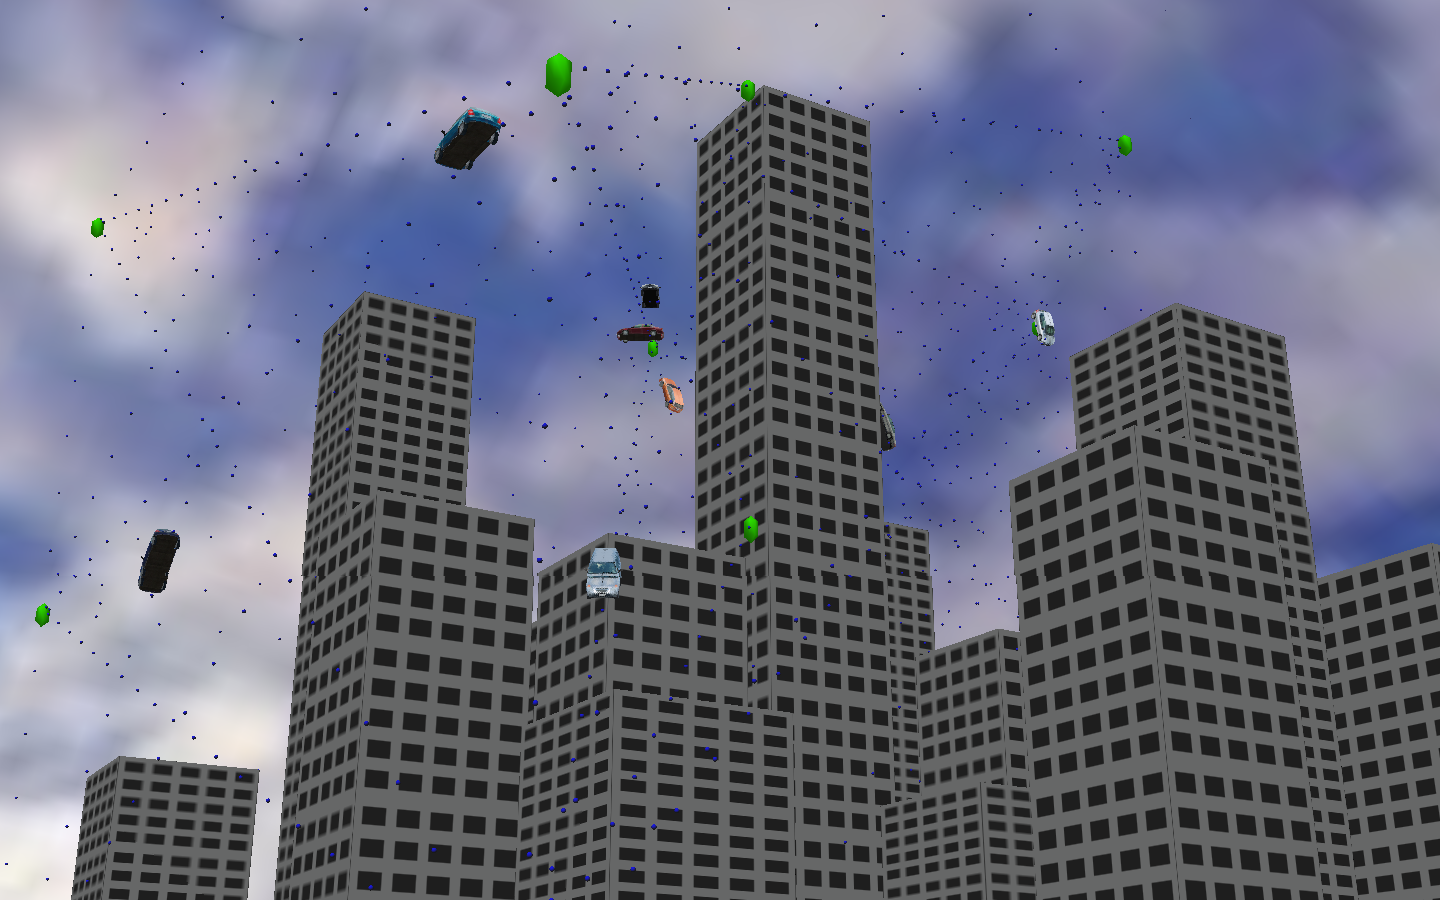
\includegraphics[width=400px]{screen.png}
	\end{center}
	\caption[]{Capture d'écran d'air traffic}
	\label{screen}
	\end{figure}
	
  \section*{Fonctionalirés}
  Sur la Figure~\ref{screen} on peut voir des objets verts qui sont des points de passage et des sphères
  bleues qui représentent les routes qui relient les waypoints. Les voitures vont forcément suivre ces routes.
  Les colisions entre les voitures ne sont pas gérées. La caméra peut-être gérée de différentes manières:
  \begin{itemize}
  \item La touche 1 permet d'avoir une caméra de type trackball (caméra par défaut)
  \item La touche 2 permet de passer en mode avion
  \item La touche 3 permet de passer en mode conduite
  \item La touche 4 permet d'avoir un manipulateur de type terrain
  \item La touche 5 permet d'avoir une caméra qui suis un chemin comme si elle était une voiture
  \end{itemize}
  Les chemins suivis par les voitures et par la caméra sont choisis aléatoirement au lancement du 
  programme. Ces chemins sont calculer de façon à ce que l'objet revienne à son point de départ à
  la fin du chemin. Une fois sont chemin terminé, l'objet recommence à le parcourir du début et il boucle
  ainsi à l'infini.

  \section*{Problèmes rencoontrés et solutions adoptées}
  Le premier problème a été la création des points de passage et des chemins possibles entre 
  ces points. En effet, il ne fallait pas que des points de passage ne se retrouve à l'intérieur ou en collision 
  avec des immeubles. Il ne fallait pas non plus que des chemins passent au travers d'immeubles. Le choix 
  des points de passage s'est fait de manière empirique. Nous avons testé des points jusqu'à trouver ceux 
  qui nous parraitssaient convenables. En utilisant tout de même des coordonnées prises sur la ville à l'aide 
  du drive manipulator. Pour les chemins, nous avons construit le graphe des liaisons possibles entre les 
  points de passage sans collision avec des immeubles en utilisant un IntersectVisitor qui nous a permis de 
  détecter quand on avait des collisions avec la ville. Les chemins des voitures sont ensuite choisit de 
  manière aléatoire dans ce graphe.
  
  Un autre problème majeur a été de faire en sorte que le voitures aient un mouvement pseudo-réaliste.
  C'est à dire qu'elles se déplacent vers l'avant et tournent pour prendre la direction du prochain point de 
  passage à chaque fois qu'elles arrivent à un point de passage. Pour calculer les matrices de rotations 
  permettant de passer d'une orientation à une autre, nous avons utiliser la fonction eulerQuat qui se sert 
  de lookAt pour avoir la direction du point a au point b en gardant le vecteur "vers le haut" voulu. Ceci afin
  que le toit de nos voitures soit autant que possible orienté vers le haut et qu'elles soient orientées dans
  la direction adéquat.

  Une autre difficulté rencontrée a été le chargement des voitures. Nous avons utilisé le fichier Car.ive
  fourni qui contenait toutefois plusieurs véhicules. Afin d'avoir de la diversité dans les voitures affichées,
  nous avons choisi de prendre aléatoirement des modèles de voiture dans ce fichier. Il a donc fallut mettre
  place la récupération aléatoire d'un noeud fils de la racine dans ce fichier.

  L'affichage des routes et des waypoints a aussi été un petit problème. Nous l'avons finalement résolu 
  en s'occupant de cet affichage lors de la création du graphe des chemins possibles. Ceci évitant un 
  parcourt complet du graph simplement pour afficher ces objets.
  
  \section*{Répartition du travail}
  Dans un premier temps Romaric c'est occupé de mettre en place la structure générale du programme,
  c'est-à-dire le main, la création de la scène avec la mise en place du skydome et le chargement d'un 
  fichier qui sera remplacé ensuite par la ville. Pendant ce temps Clément s'est chargé de créer le modèle
  3D de la ville. Une fois cette base en place, Clément s'est chargé de choisir aléatoirement une voiture dans
  le fichier Car.ive et nous avons alors réfléchit à la façon d'animer ces dernières. Nous avons alors choisit de
  créer dynamiquement un graphe entre des points de passage. Après que l'on ait trouvé les pistes pour
  effectuer cette tâche, Clément s'est occupé de créer le graphe et Romaric s'est occuper d'afficher les
  points de passage et les routes possibles entre ces points. Il a aussi recherché un ensemble de points 
  possibles pour les points de passage. Clément a ensuite fait une première version de la création 
  automatique de chemin pour les voitures avec des rotations pseudo-réalistes qui sera ensuite revu par
  Romaric afin d'en retirer les quelques beugs. Enfin Romaric s'est occupé du placement par défaut de la
  caméra et de faire en sorte que l'on puisse suivre un chemin comme si l'on était une voiture à l'aide de la 
  caméra.

  \section*{Conclusion} 
  Au cours de ce projet nous avons découvert la fléxibilité d'OpenSceneGraph en choisissant un projet libre.
  En effet nous avons trouvé intéressant de générer facilement des routes de façon dynamique afin d'en
  animer des véhicules. Il est aussi très simple de parcourir un arbre pour en retirer les modèles souhaités.
  De plus il permet le chargement de modèles 3D existant et la manipulation de ces objets à assez haut 
  niveau de façon assez simple. Grâce au graph de scène, on peut rapidement réaliser une scène d'une 
  complexité moyenne. OpenSceneGraph est donc un outil intéressant si l'on souhaite créer rapidement des 
  scenes 3D sans se soucier directement des problématiques de bas niveau de la 3D. Il est de plus assez 
  puissant et performant grâce aux algorithmes d'élimination des noeuds et faces invisibles. C'est donc un 
  outil auquel il faut penser si l'on souhaite modéliser un environnement 3D en ne s'occupant que de la 
  disposition des objets et de leurs interactions et en laissant le rendu à la bibliothèque.

\end{document}
